\subsection{M-array Pattern Projection Method \cite{morita1988reconstruction}}

The binary M-array pattern projection method consists in projecting dark and light dots. The color of each dot represents a 0 (dark) or 1 (light) of the M-array pattern. The spatial coordinates of each observed dot matched with one of the initial pattern can be determined by triangulation. However, pattern disorders occur often in the observed pattern and some dots cannot be matched. One of the asset of this method is the detection and correction of pattern disorders.

\subsubsection{Pattern Disorders}
\label{PatternDisorders}
According to \cite{morita1988reconstruction}, there are three different types of pattern disorder.
\begin{itemize}
\item Loss of dots. If there are several objects in the scene, an object may obstruct the pattern. The first, second and third dots on the figure \ref{fig:disorder1}, are not visible by the camera on figure \ref{fig:disorder2}.
\item Displacement of dots : in comparison to the initial pattern projected, the dots may shift because of the depth of each object. On the figure \ref{fig:disorder1}, the dots 4 to 6 on the object 2 have shifted to the left compared with the dots of object 1.
\item Interchange of dots : if an object is in front of another, the order of dots may change. The third dot on figure \ref{fig:disorder1} has changed of order and is the fourth one from the point of view of the camera (figure \ref{fig:disorder2}).
\end{itemize}

\begin{figure}[!h] 
\centering
\subfigure[]{
  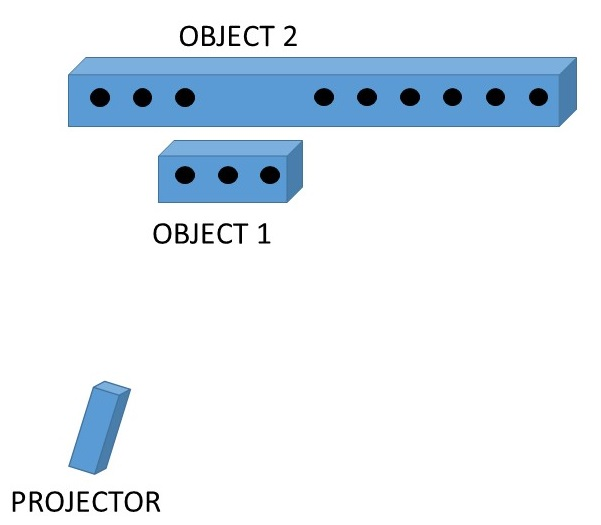
\includegraphics[scale=0.42]{fig/disorder1.jpg}
  \label{fig:disorder1}
}
\quad 
\subfigure[]{
  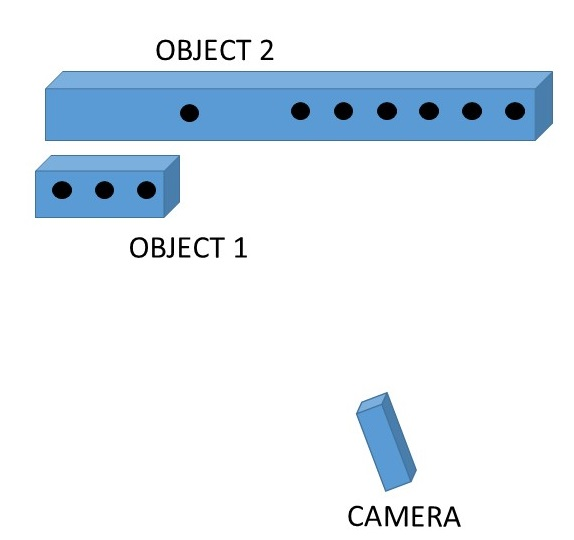
\includegraphics[scale=0.42]{fig/disorder2.jpg}
  \label{fig:disorder2}
}
\caption{Pattern Disorders}
\end{figure}






\subsubsection{Correction of Pattern Disorders}
There are four steps in the matching of the observed dots with those of the pattern and the correction of the pattern disorders.





\paragraph*{Temporary Array}
~~\\
The image recorded is analyzed row by row of dots and a 2-D array which contains the numbers of the observed dots is created. This array will be used to differentiate each dot. The array can be computed by these steps :
\begin{itemize}
\item Creation of the array (the elements are initialized to zero).
\item Scan of the image to detect dots. Each time a point is detected, its value and location (center) are saved into 1-D arrays VALUE, X and Y.
\item The position of the dots are quantized according to the initial pattern using X and Y so that adjoining dots have successive quantized coordinates.
\item Insertion of the number of each dot into the array (the location into the array corresponds to the quantized coordinates).
\end{itemize}

This temporary array (T-array) may have some vacant places due to disorder pattern.

\paragraph*{Grow}
~~\\
Each element of the T-array gets an index (column number of the M-array). To do so, a window is defined and applied to the T-array and the M-array where the elements into the window of each array have the same value. The element into the window of the T-array can be indexed using the M-array and the two windows moved simultaneously by one column or row. This is repeated until a difference between the two windows is detected. New windows are then initialized elsewhere. The grow terminate when no window can be initialized to an area of the T-array where there is no index yet.


\paragraph*{Detection of Pattern Disorders}
~~\\
The detection step is carried out during the growing and is explained below using an example. We use a 3$\times$4 window.
\begin{itemize}
\item step 1 : the region growing starts at (0',0') and (0,0) on the T-array and M-array (see Figure \ref{fig:detect} a).
\item step 2 : the window slides to the right until a difference between the two arrays is detected (see Figure \ref{fig:detect} b).
\item step 3 : In the T-array, the window is shifted to the right until the error is on the left side of the window. In the M-array, the window is displaced until it matches with the one of the T-array (see Figure \ref{fig:detect} c).
\item step 4 : the windows now slides to the left and all the indices of the columns of the T-array are readjusted according to the two windows until another difference is detected.
\end{itemize}

\begin{figure}[h]
	\centering
	\hspace*{-2cm}
   \begin{minipage}[b]{0.50\linewidth}
      \centering 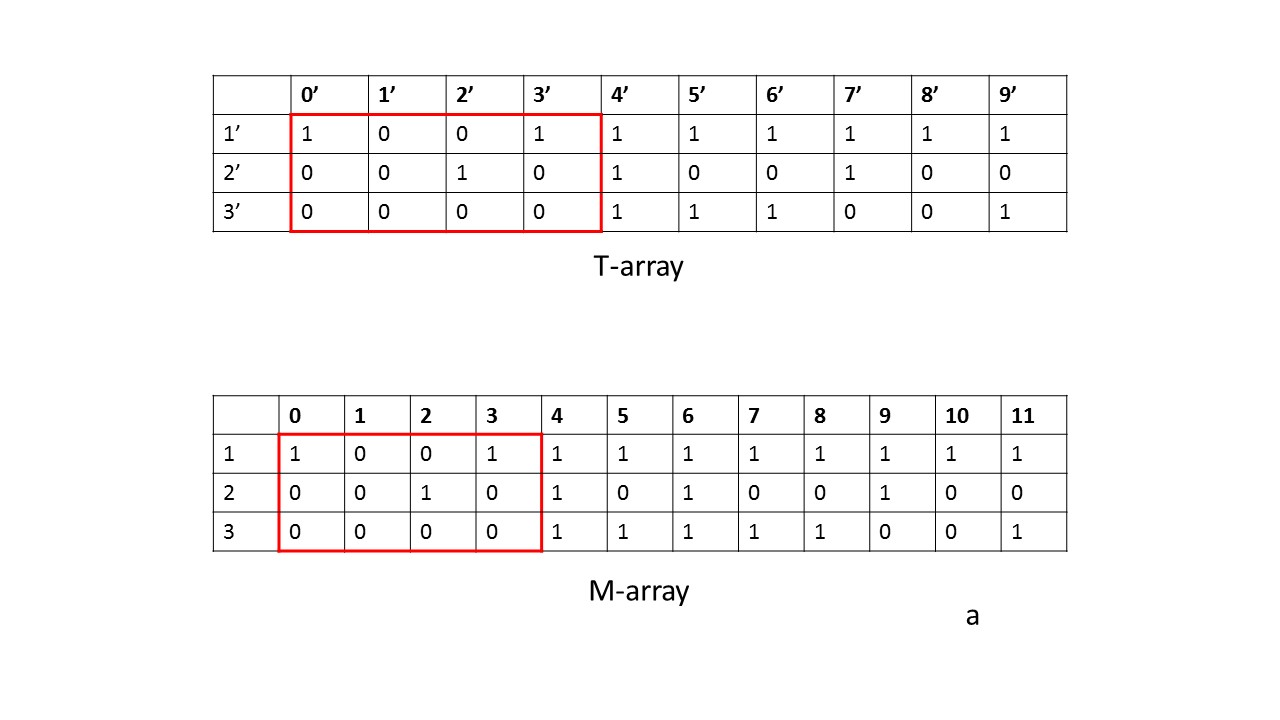
\includegraphics[scale=0.3]{fig/detect1.jpg}
      %\caption{\it Legend 1}
   \end{minipage}\hfill
   \begin{minipage}[b]{0.50\linewidth}   
      \centering 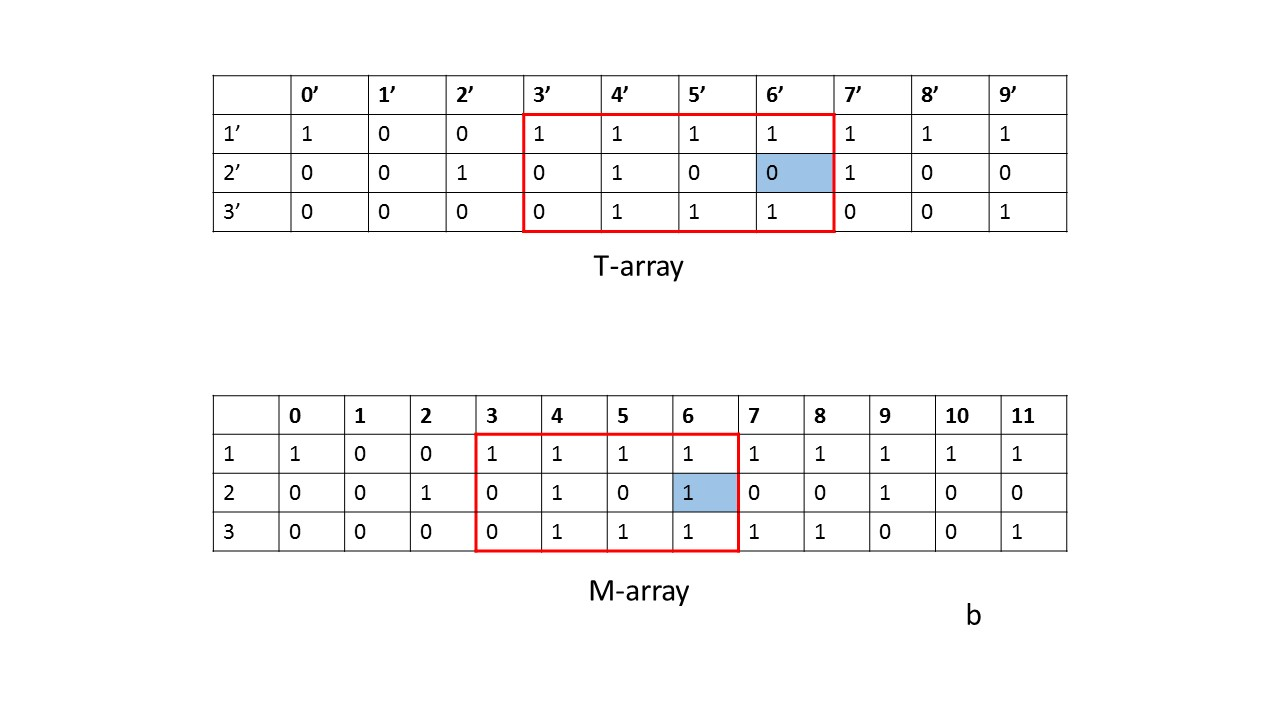
\includegraphics[scale=0.3]{fig/detect2.jpg}
      %\caption{Legend 2}
   \end{minipage}
	\hspace*{-2cm}
   \begin{minipage}[b]{0.50\linewidth}
      \centering 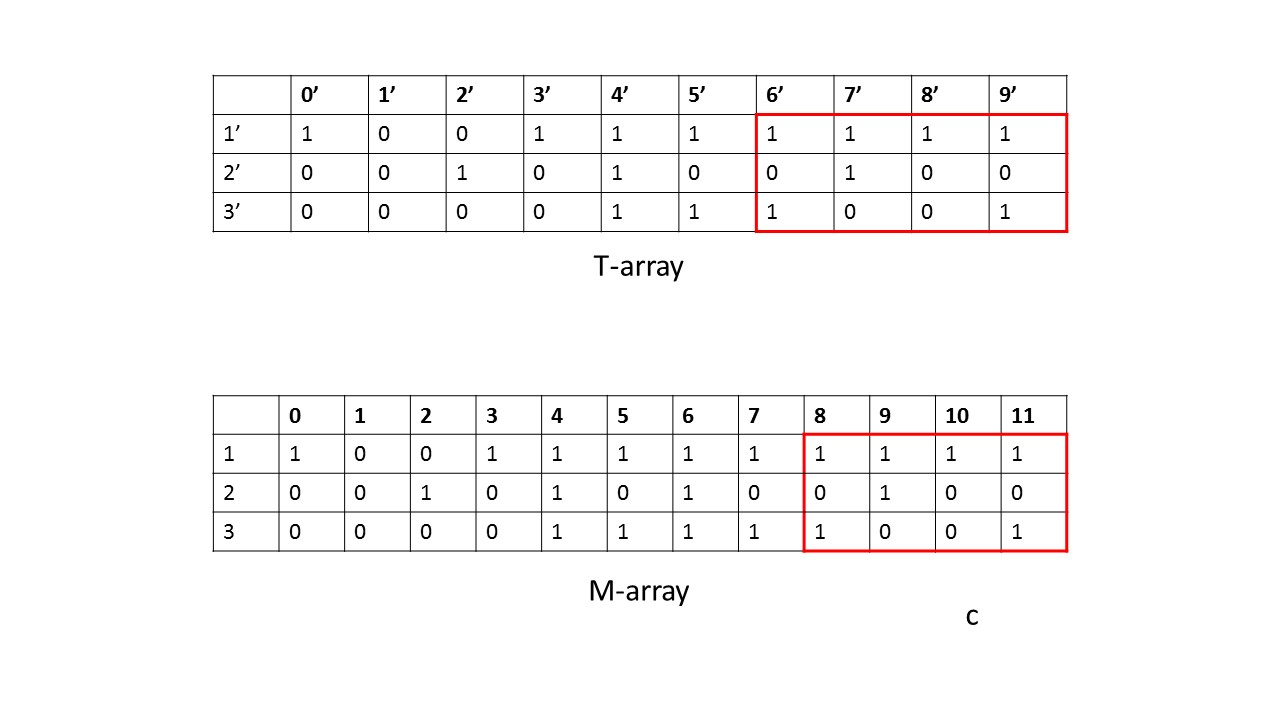
\includegraphics[scale=0.3]{fig/detect3.jpg}
      %\caption{Legend 3}
   \end{minipage}\hfill
   \begin{minipage}[b]{0.50\linewidth}   
      \centering 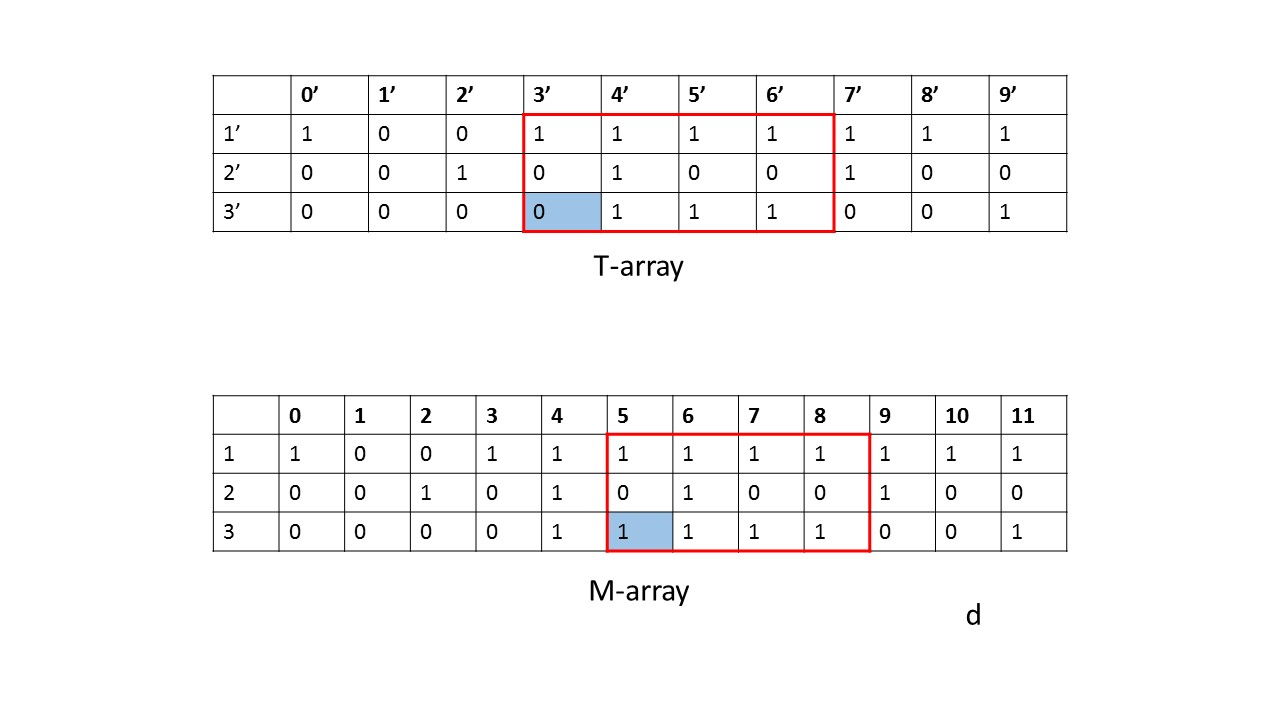
\includegraphics[scale=0.3]{fig/detect4.jpg}
     % \caption{Legend 4}
   \end{minipage}
	\caption{Detection of the disorders}
	\label{fig:detect}
\end{figure}


Then, as regions of the T-array extends because of the step 4, a new window may be initialized on the extended region and the growing starts once more. At the end, except some array cells corresponding to dots lighted near the border of two objects, all the indices of the T-array have been determined.










\paragraph*{Correction of Pattern Disorders}
~~\\
Knowing that, in the T-array, the elements which still have no indices appear to be mostly alone or consecutive, some rules permit to correct the index of these elements.

\begin{itemize}
\item if the element above and the one below have the same index k, the current element has also this index k.
\item if the element at the left has the index k-1 and the one at the right k+1, then the current element has the index k.
\item the difference between the index of two horizontal neighbors corresponding to closer positions on the image is one.
\item if the indices of a vertical sequence are still undetermined, they get the index of the element at the top or bottom of the vertical.

\item if the indices of an consecutive horizontal sequence are still undetermined, they get the index such as it increases by one from index determined on the left to the one on the right.
\begin{tabular}{|*{11}{c|}}
    \hline
     k-5  & k-4  & k-3  & \textcolor[rgb]{1,0,0}{k-2}  & \textcolor[rgb]{1,0,0}{k-1}  & \textcolor[rgb]{1,0,0}{k}  & \textcolor[rgb]{1,0,0}{k+1}  & k+2  & k+3  & k+4 & k+5 \\
    \hline
\end{tabular}
\end{itemize}

According to \cite{morita1988reconstruction}, the previous rules should correct the most of the errors of indexation and the cases where the error cannot be corrected are scarce.







\subsection{Grid Indexing}

The method of the binary M-array projection is based on the matching of a binary array, but other patterns can be used too to permit the matching of the projected and observed patterns. A non-exhaustive list of grid indexing is presented below.

\subsubsection{Mini-patterns Used as Code Words}

Instead of using a binary array, an array of words coded by patterns can be employed. Each pattern codes a word. As instance, on the figure \ref{fig:codeWords}, three words have been coded and permit to convert the projected pattern into a array of integers.


\begin{figure}[h!]
  %\centering
  \centerline{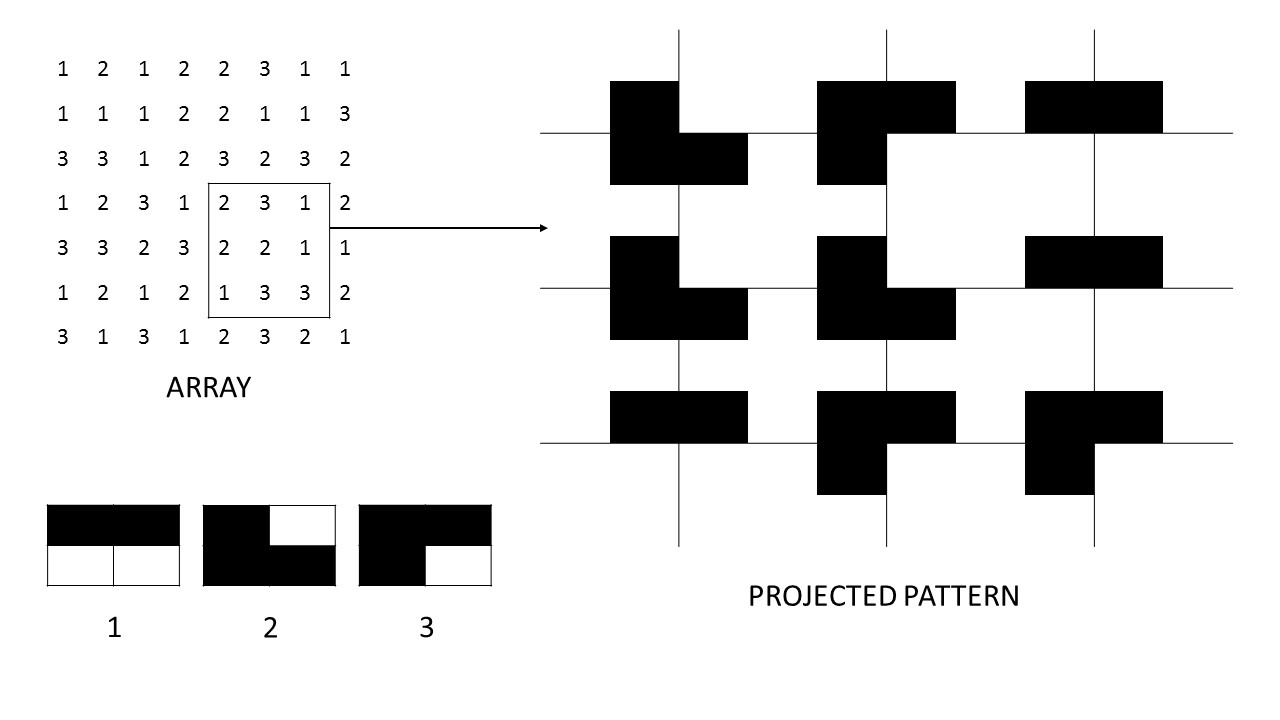
\includegraphics[scale=0.48]{fig/codeWords.jpg}}
  \caption{Mini-pattern used as code words}
  \label{fig:codeWords}
\end{figure}





\subsubsection{2D Array of Color-coded Dots}

An other technique is the 2D array of color-coded dots. The concept of this method is almost the same as the previous one but instead of using pattern to code a word, colors are manipulated (see Figure \ref{fig:color-coded}).

\begin{figure}[h]
  %\centering
  \centerline{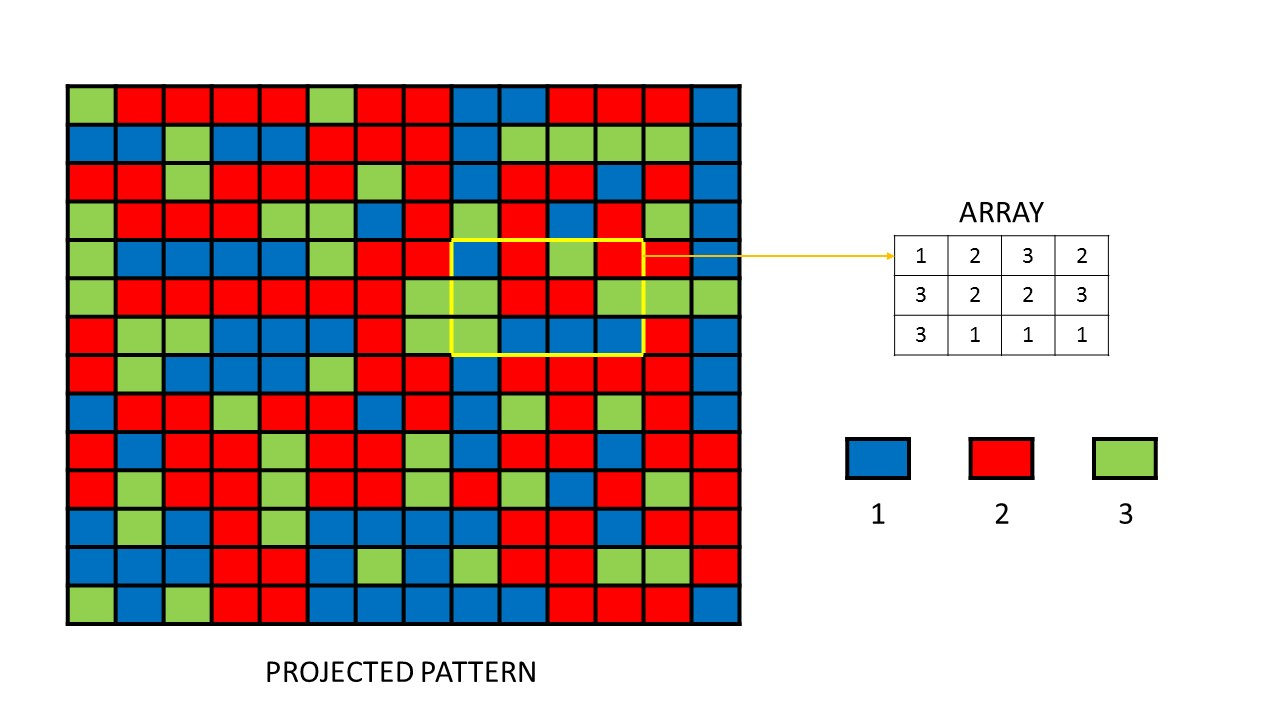
\includegraphics[scale=0.5]{fig/color-coded.jpg}}
  \caption{2D Array of Color-coded Dots}
  \label{fig:color-coded}
\end{figure}
